%%%%%%%%%%%%%%%%%%%%%%%%%%%%%%%%%%%%%%%%%%%%%%%%%%%%%%%%%%%%%%%%%%%%%
% LaTeX Template: Project Titlepage Modified (v 0.1) by rcx
%
% Original Source: http://www.howtotex.com
% Date: February 2014
% 
% This is a title page template which be used for articles & reports.
% 
% This is the modified version of the original Latex template from
% aforementioned website.
% 
%%%%%%%%%%%%%%%%%%%%%%%%%%%%%%%%%%%%%%%%%%%%%%%%%%%%%%%%%%%%%%%%%%%%%%

\documentclass[12pt]{report}
\usepackage[a4paper]{geometry}
\usepackage[myheadings]{fullpage}
\usepackage{fancyhdr}
\usepackage{lastpage}
\usepackage{graphicx, wrapfig,setspace, booktabs}
\usepackage[T1]{fontenc}
\usepackage[font=small, labelfont=bf]{caption}
\usepackage{fourier}
\usepackage[protrusion=true, expansion=true]{microtype}
\usepackage[english]{babel}
\usepackage{sectsty}
\usepackage{lipsum}
\usepackage[hyphens]{url}
%\usepackage{subfig}
\usepackage{hyperref}
\usepackage{alphalph}
\usepackage[utf8]{inputenc}
\usepackage{multicol}
\usepackage{amsmath}
\usepackage{subfigure}
\renewcommand*{\thesubfigure}{%
\alphalph{\value{subfigure}}%
}%


\newcommand{\HRule}[1]{\rule{\linewidth}{#1}}
\onehalfspacing
\setcounter{tocdepth}{5}
\setcounter{secnumdepth}{5}
\usepackage{float}

\usepackage[backend=bibtex,style=chem-acs,biblabel=dot]{biblatex}
\addbibresource{references.bib}

%-------------------------------------------------------------------------------
% HEADER & FOOTER
%-------------------------------------------------------------------------------
\pagestyle{fancy}
\fancyhf{}
\setlength\headheight{15pt}
\fancyhead[L]{CS7015: PA4}
\fancyhead[R]{Deep Learning}
\fancyfoot[R]{Page \thepage\ of \pageref{LastPage}}
%-------------------------------------------------------------------------------
% TITLE PAGE
%-------------------------------------------------------------------------------

\begin{document}

\title{ \normalsize \textsc{ID7123 : Center for Computational Brain Research}
		\\ [2.0cm]
		\HRule{0.5pt} \\
		\LARGE \textbf{\uppercase{Multi-Armed Bandits}}\\
        \large{- Prof. Prashanth L. A. -}
		\HRule{2pt} \\ [0.5cm]
		\normalsize \date{20 January 2019} \vspace*{5\baselineskip}}



\author{
		Student ID:  \\ 
		Ganga Meghanath \\
		EE15B025
		}

\renewcommand\thesection{\arabic{section}}
\maketitle
\tableofcontents
\newpage

%-------------------------------------------------------------------------------
% Section title formatting
\sectionfont{\scshape}
%-------------------------------------------------------------------------------

%-------------------------------------------------------------------------------
% BODY
%-------------------------------------------------------------------------------

\section{Introduction}
In a ``Multi-armed Bandit problem'', a person must choose between multiple actions (originally comes from the idea of slot machines, the "one-armed bandits"), each with an unknown reward. The goal is to determine the best or most profitable outcome through a series of choices. At the beginning of the experiment, when odds and payouts are unknown, the gambler must determine which machine to pull, in which order and how many times. \\

\noindent Here, we have been provided with the following scenario :
\begin{table}[H]
  \centering
  \begin{tabular}{ | c | c | c | c | c | c | c | c | c | c | c |}
    \hline
    \textbf{Arms} & \textbf{1} & \textbf{2} & \textbf{3} & \textbf{4} & \textbf{5} & \textbf{6} & \textbf{7} & \textbf{8} & \textbf{9} & \textbf{10}\\ 
    \hline
    P1 & B(0.6) & B(0.4) & B(0.4) & B(0.4) & B(0.4) & B(0.3) & B(0.3) & B(0.3) & B(0.3) & B(0.3)\\
    \hline
    P2 & B(0.62) & B(0.6) & B(0.6) & B(0.6) & B(0.6) & B(0.58) & B(0.58) & B(0.58) & B(0.5) & B(0.5)\\
    \hline
    P3 & B(0.8) & B(0.4) & B(0.3) & B(0.2) & B(0.1) & & & & &\\
    \hline
    P4 & U(20) & U(16) & U(12) & & & & & & &\\
	\hline
  \end{tabular}
\end{table}

\noindent where B stands for \textit{Bernoulli distribution} with $p$-value inside the bracket and U stands for \textit{Uniform distribution} with lower limit 0 and upper limit in brackets.\\

\noindent Here 2 algorithms have been portrayed :

	\subsection{Upper Confidence Bound (UCB)} 
		\begin{table}[H]
  			\centering
  			\begin{tabular}{ | c |}
    		\hline
    		\noindent Initialization: Play each arm once,\\
    		\noindent \textbf{For} t = K + 1, \dots , n, \textbf{repeat}\\
    		(1) Play arm $I_t = arg max_{k=1,...,K} UCB_t(k)$, where \\
    		$UCB_t(k) = \hat{\mu}_k(t-1) + \sqrt{\frac{8 \log t}{T_k (t-1)}}$\\
    		(2) Observe sample $X_t$ from the distribution $P_{I_{t}}$ corresponding to the arm $I_t$.\\
    		\hline
			\end{tabular}
		\end{table}
		
	\subsection{Explore-then-Commit (ETC)}
		\begin{table}[H]
  			\centering
  			\begin{tabular}{ | c |}
    		\hline
    		(1)  \textbf{Exploration phase:} During rounds 1, \dots , mK, play \\
    		each arm m times.\\
    		(2) \textbf{Exploitation phase:} During the remaining (n - mK) rounds, \\
    		play the arm with the highest empirical mean reward, i.e.,\\
    		 $arg max_{k=(1,\dots,K)} \hat{µ}_k(mK)$.\\
    		\hline
			\end{tabular}
		\end{table}

		\noindent For \textbf{Gap-dependent bound for ETC}, the regret bound for horizon $n$ is given by,
		\begin{equation}
			R_n \leq m \sum_{i=1}^K \Delta_i + (n - mK) \sum_{i=1}^K \Delta_i \exp \Big( \frac{-m \Delta^2}{4} \Big)
		\end{equation}  
		where $m$ is the number of times each arm is played during the \textit{exploration phase} and the $\Delta$ values are given by :
		\begin{table}[H]
  			\centering
  			\begin{tabular}{ | c | c | c | c | c | c | c | c | c | c | c |}
    			\hline
   	 			\textbf{Arms} & \textbf{1} & \textbf{2} & \textbf{3} & \textbf{4} & 					\textbf{5} & \textbf{6} & \textbf{7} & \textbf{8} & \textbf{9} & \textbf{10}\\ 
			    \hline
			    P1 & 0 & 0.2 & 0.2 & 0.2 & 0.2 & 0.3 & 0.3 & 0.3 & 0.3 & 0.3\\
    			\hline
    			P2 & 0 & 0.02 & 0.02 & 0.02 & 0.02 & 0.04 & 0.04 & 0.04 & 0.12 & 0.12\\
    			\hline
    			P3 & 0 & 0.4 & 0.5 & 0.6 & 0.7 & & & & &\\
    			\hline
    			P4 & 0 & 2 & 4 & & & & & & &\\
				\hline
  			\end{tabular}
		\end{table}

		\noindent which were calculated as $\Delta_i = \mu_\star - \mu_i$ and in the above scenario, $1^{st}$ arm is optimal (max $\mu$).



%-------------------------------------------------------------------------------
%Experiments
%-------------------------------------------------------------------------------
\section{Experiments}
	For the purpose of experiments, use the folder which is structured as :
	\begin{itemize}
		\item Multi-Armed-Bandit
		\begin{itemize}
			\item Report
			\begin{itemize}
				\item .tex file and compilatoin files
				\item Figures : Plotted figures are saved here
			\end{itemize}
			\item main.py : Main function
			\item alg.py : Contains ETC and UCB algorithms
			\item plot.py : Contains the plotting functions
			\item constants.py : Contains values such as horizon, distribution, etc
			\item sampler.py : Contains the sampling distributions
		\end{itemize}
	\end{itemize}
	
	\noindent The \textbf{command line arguments} are given as follows,
	\begin{enumerate}
		\item --distribution :
		\begin{itemize}
			\item default="P1"
			\item type = str
			\item help='Choose from P1, P2, P3, P4'
		\end{itemize}		

    	\item --algorithm : 
    	\begin{itemize}
    		\item default="ETC" 
            \item type = str
            \item help='Choose from ETC, UCB'
    	\end{itemize}
                        
		\item --m :
		\begin{itemize}
			\item default=300
            \item type = int
            \item help='Int value : no. of times to explore each arm for ETC'
		\end{itemize}
                        
    	\item --err :
    	\begin{itemize}
    		\item default=1
            \item type = int
            \item help='Int value : interval for error bar'
    	\end{itemize}
                        
		\item --compare :
		\begin{itemize}
		 	\item default=False
            \item type = bool
            \item help='Whether to compare different algorithms'
		\end{itemize}                 
	\end{enumerate}
	
	\noindent For running the code, example commands are : 
	\begin{enumerate}
		\item python main.py --distribution P1 --algorithm UCB
		\item python main.py --distribution P3 --algorithm ETC --m 109
		\item python main.py --distribution P3 --compare True
	\end{enumerate}
	
	\noindent \textbf{NOTE :} For finding the \textbf{optimal} $\boldsymbol{m}$ values for \textbf{ETC}- algorithm, an online plotting resource called \textit{Desmos-Graphing Calculator} has been used to plot \textbf{Eq(1)} where \underline{m is replaced by x}.\\
	
	\noindent Also note that the error bars aren't visible in the figures for percentage of optimal arm pulled for ETC because the errors are extremely small across the experiments ($\sim 2.27e-13$). This is because, while using the optimal m, beyong the point, in almost all the experiments, we exploit the optimal arm and hence there is no variation before and after identification of an optimal arm (since the experimentally found best arm is the actual optimal arm).
	
	\subsection{P1 set of Arms}
		\subsubsection{Explore-then-Commit (ETC)}
			For this set of arms, the optimal value of $m$ was found to be 334 and the minimum value of the maximum regret was observed to be 962.45 at the minima of the graph as can be seen from the figure below. It was plotted using the equation:
			$$x\cdot\left(0.8+1.5\right)+\left(10000-x\cdot10\right)\left(0.8\cdot e^{-x\cdot0.01}+1.5\cdot e^{-x\cdot\frac{0.09}{4}}\right)$$
			
			\begin{figure}[H]
				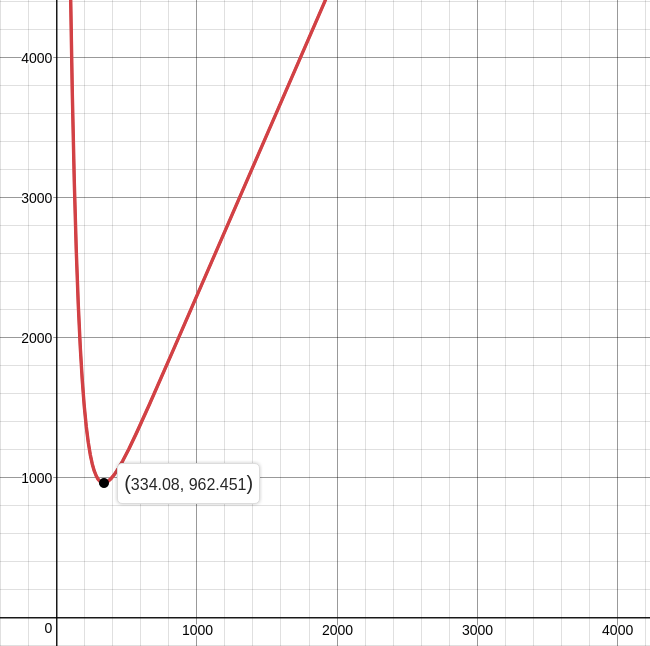
\includegraphics[scale=0.5]{Figures/m_P1.png}
			\end{figure}
			
			\begin{figure}[H]
				\begin{multicols}{2}
					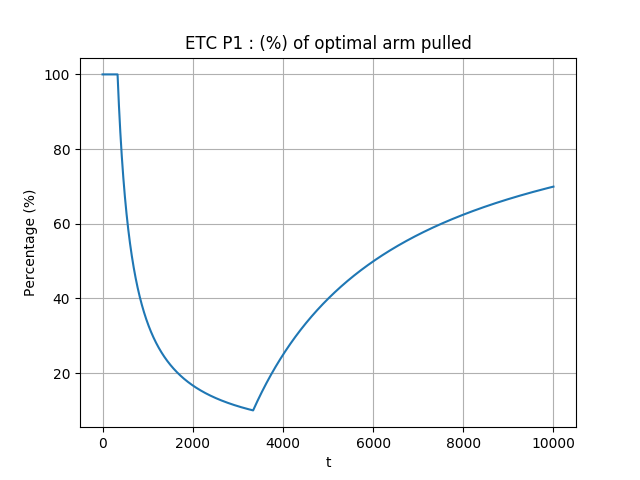
\includegraphics[scale=0.5]{Figures/ETC_P1_334_op.png} \par
					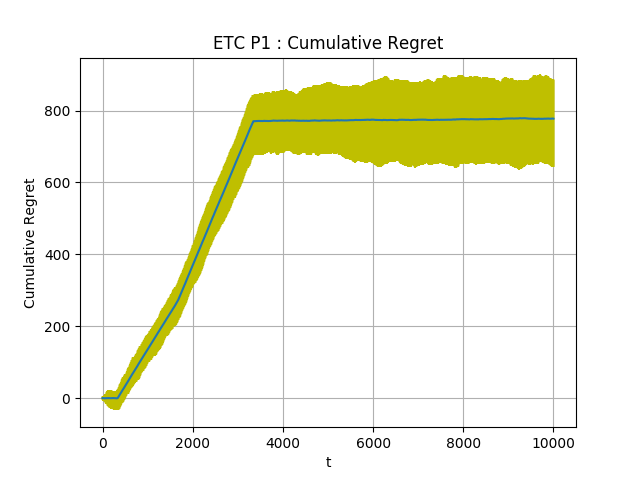
\includegraphics[scale=0.5]{Figures/ETC_P1_334_ret.png}
				\end{multicols}
				\caption{Evaluation plots for ETC for P1 set of arms}
				\label{Fig1}
			\end{figure}
				
		\subsubsection{Upper Confidence Bound (UCB)}
			\begin{figure}[H]
				\begin{multicols}{2}
					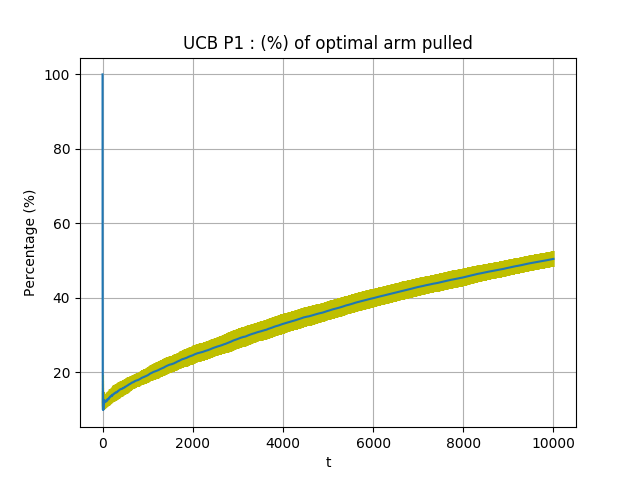
\includegraphics[scale=0.5]{Figures/UCB_P1_op.png} \par
					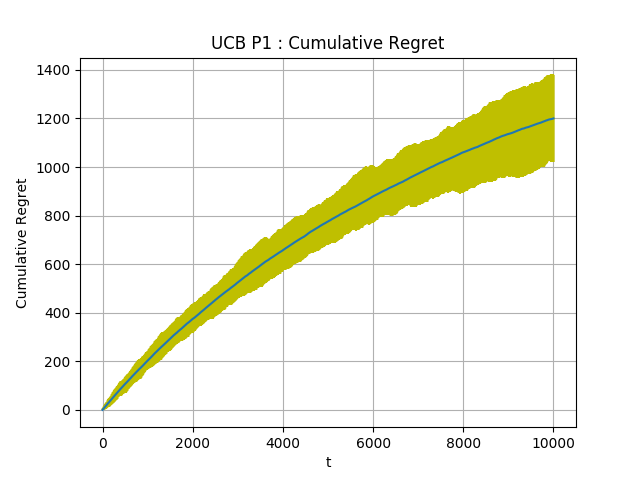
\includegraphics[scale=0.5]{Figures/UCB_P1_ret.png}
				\end{multicols}
				\caption{Evaluation plots for UCB for P1 set of arms}
				\label{Fig2}
			\end{figure}

	\noindent On comparison, we see that at t=n, the percentage of optimal arms pulled by using ETC surpasses UCB by around $20\%$	and the final cumulative regret of ETC exceeds UCB by around a value of 450. In terms of the percentage of optimal arms pulled and the cumulative return at the end of the horizon using optimal $m$ value, ETC seems to be performing better.
	
	\subsection{P2 set of Arms}
		\subsubsection{Explore-then-Commit (ETC)}
			For this set of arms, the optimal value of $m$ was found to be 1474 and the minimum value of the maximum regret was observed to be 0 before the minima of the graph as can be seen from the figure below. It was plotted using the equation:
				$$x\cdot\left((4\cdot0.02+3\cdot0.04+2\cdot0.12\right)+\left(10000-x\cdot10\right)\cdot\left(4\cdot0.02\cdot e^{-x\cdot\frac{0.02^2}{4}}+3\cdot0.04\cdot e^{-x\cdot\frac{0.04^2}{4}}+2\cdot0.12\cdot e^{-x\cdot\frac{0.12^2}{4}}\right)$$
			
			\begin{figure}[H]
				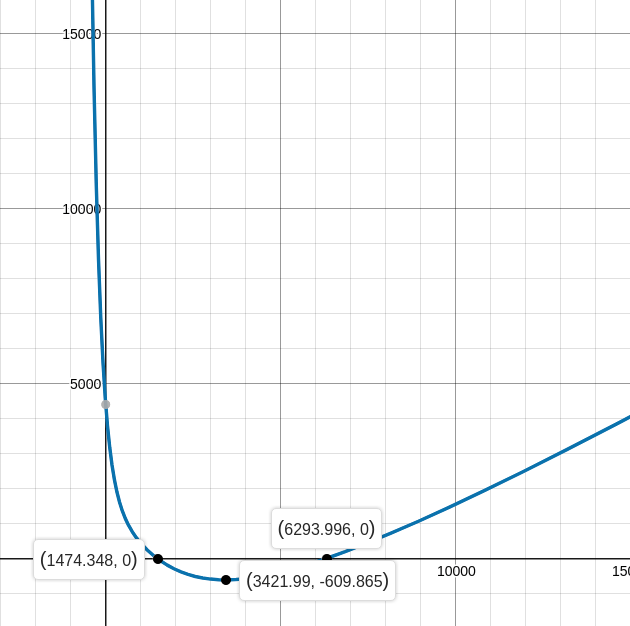
\includegraphics[scale=0.5]{Figures/m_P2.png}
			\end{figure}
			
			\noindent Here, there seems to be something oddly wrong. On plotting, the regret takes negative values. This means that the horizon is not sufficient enough for us to find an optimal m. Hence, there seems to be a need to increase the horizon and recalculate the optimal m value and conduct the experiment. Since the horizon here is fixed at n=10000, we won't be proceeding with ETC algorithm by finding optimal m value.
			
		\subsubsection{Upper Confidence Bound (UCB)}
			\begin{figure}[H]
				\begin{multicols}{2}
					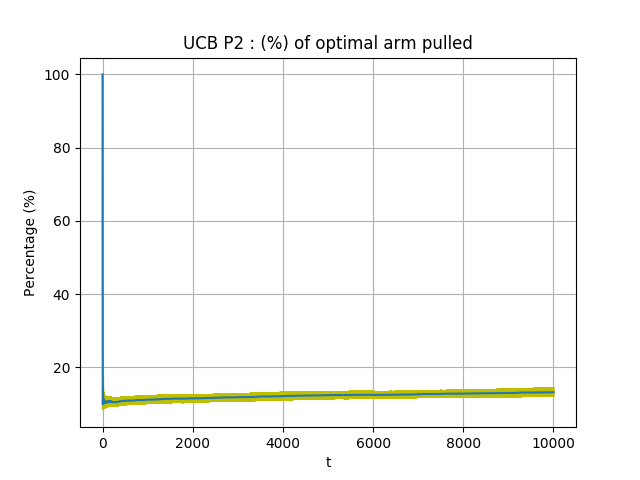
\includegraphics[scale=0.5]{Figures/UCB_P2_op.png} \par
					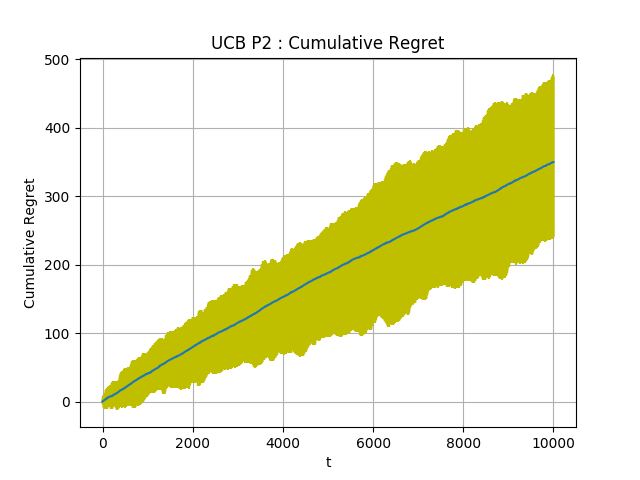
\includegraphics[scale=0.5]{Figures/UCB_P2_ret.png}
				\end{multicols}
				\caption{Evaluation plots for UCB for P2 set of arms}
				\label{Fig3}
			\end{figure}
			
			\noindent As can be seen from the above figures, UCB seems to be performing quite poorly on this set of ditributions for the arms where the actual mean values are very close to each other. UCB seems to be stuck in local minimas and hence the percentage of optimal arm pulled doesn't cross $15\%$ at the end of the horizon. As for the regret, it's almost linear because the difference keeps increasing, ie., the cumulative regret keeps increasing. This is because the algorithm is stuck using sub-optimal solutions. If the difference between the mean values were larger, then we could hope for better performance of the algorithm. (Note that we're using bernoulli distribution for each arm here. This makes the problem of small differences between the mean values worse.)
			
	\subsection{P3 set of Arms}
		\subsubsection{Explore-then-Commit (ETC)}
			For this set of arms, the optimal value of $m$ was found to be 109 and the minimum value of the maximum regret was observed to be 290.54 at the minima of the graph as can be seen from the figure below. It was plotted using the equation:
			$$x\cdot\left(0.4+0.5+0.6+0.7\right)+\left(10000-x\cdot10\right)\cdot\left(0.4\cdot e^{-x\cdot\frac{0.4^2}{4}}+0.5\cdot e^{-x\cdot\frac{0.5^2}{4}}+0.6\cdot e^{-x\cdot\frac{0.6^2}{4}}+0.7\cdot e^{-x\cdot\frac{0.7^2}{4}}\right)$$
			
			\begin{figure}[H]
				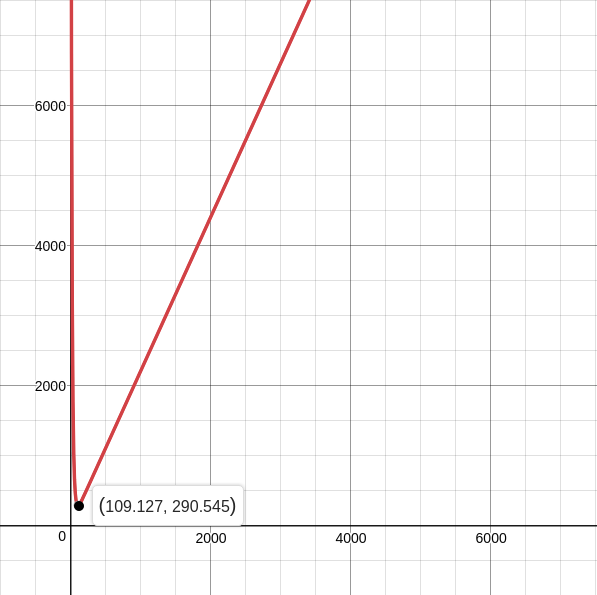
\includegraphics[scale=0.5]{Figures/m_P3.png}
			\end{figure}
			
			\begin{figure}[H]
				\begin{multicols}{2}
					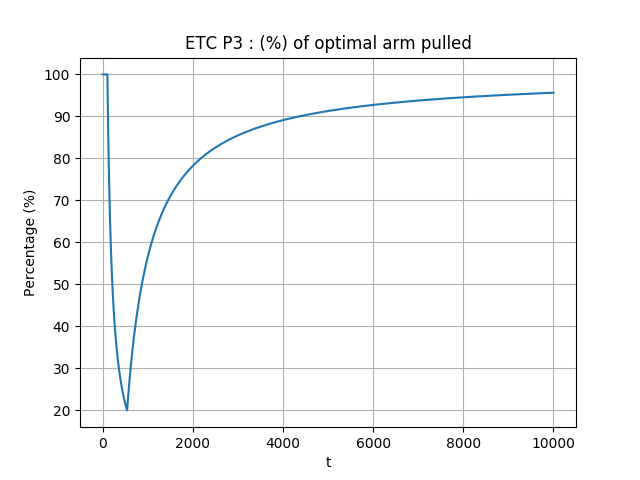
\includegraphics[scale=0.5]{Figures/ETC_P3_109_op.png} \par
					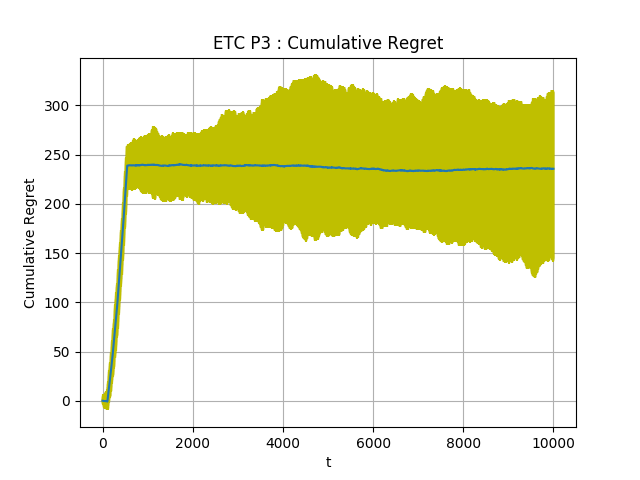
\includegraphics[scale=0.5]{Figures/ETC_P3_109_ret.png}
				\end{multicols}
				\caption{Evaluation plots for ETC for P3 set of arms}
				\label{Fig4}
			\end{figure}
				
		\subsubsection{Upper Confidence Bound (UCB)}
			\begin{figure}[H]
				\begin{multicols}{2}
					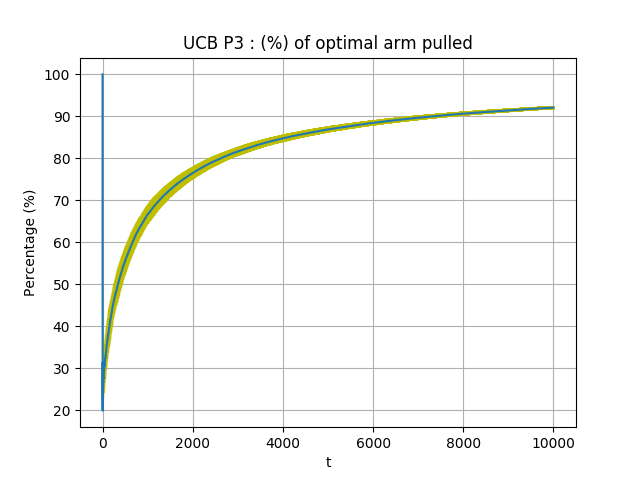
\includegraphics[scale=0.5]{Figures/UCB_P3_op.png} \par
					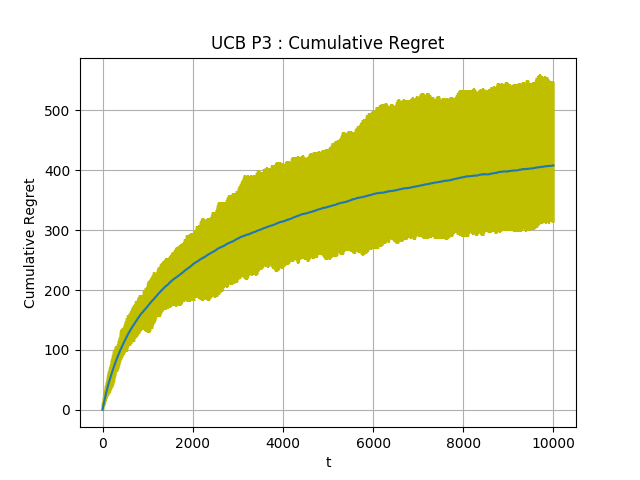
\includegraphics[scale=0.5]{Figures/UCB_P3_ret.png}
				\end{multicols}
				\caption{Evaluation plots for UCB for P3 set of arms}
				\label{Fig5}
			\end{figure}
			
		\noindent On comparison, we see that at t=n, the percentage of optimal arms pulled by using ETC exceeds UCB only by around $3\%$ but the final cumulative regret of UCB exceeds ETC by around a value of 170. So both algorithms seems to be performing sort of equally at the end of the horizon in this case, using optimal m for ETC.	But final cumulative return of UCB is higher.
		
	\subsection{P4 set of Arms}
		\subsubsection{Explore-then-Commit (ETC)}
			For this set of arms, the optimal value of $m$ was found to be 8 and the minimum value of the maximum regret was observed to be 54.6 at the minima of the graph as can be seen from the figure below. It was plotted using the equation:
			$$x\cdot\left(2+4\right)+\left(10000-x\cdot10\right)\cdot\left(2\cdot e^{-x\cdot\frac{2^2}{4}}+4\cdot e^{-x\cdot\frac{4^2}{4}}\right)$$
			
			\begin{figure}[H]
				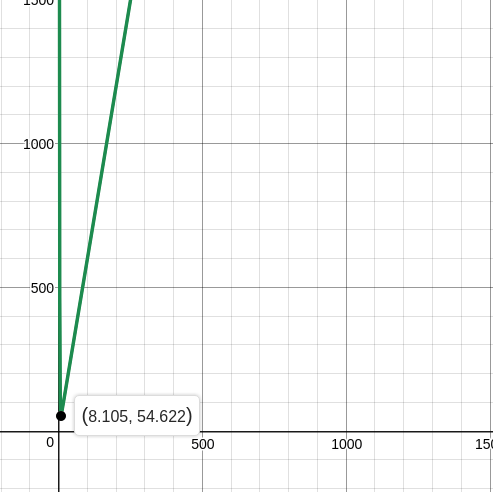
\includegraphics[scale=0.5]{Figures/m_P4.png}
			\end{figure}
			
			\begin{figure}[H]
				\begin{multicols}{2}
					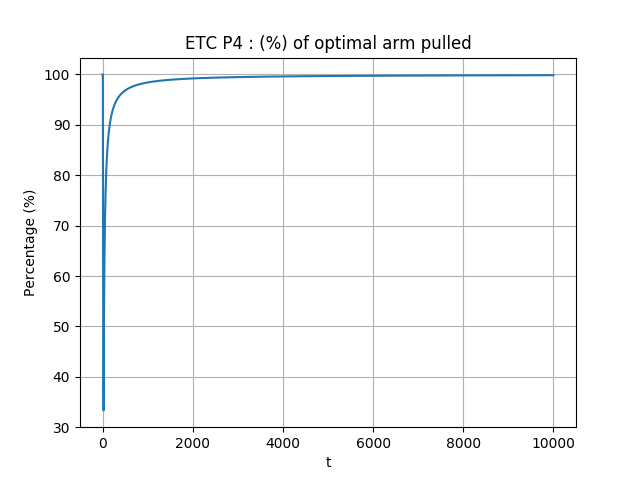
\includegraphics[scale=0.5]{Figures/ETC_P4_8_op.png} \par
					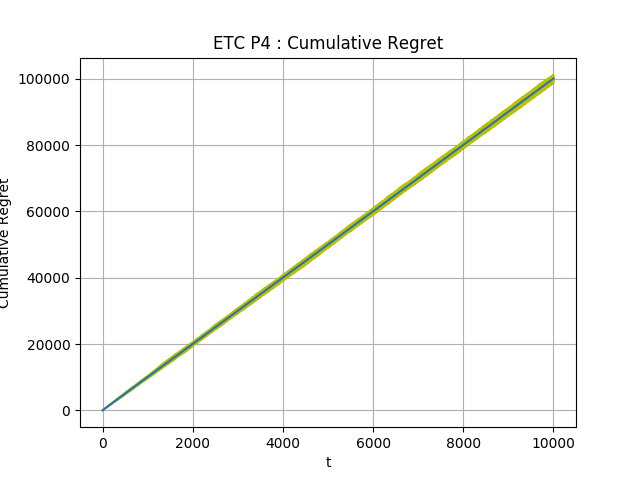
\includegraphics[scale=0.5]{Figures/ETC_P4_8_ret.png}
				\end{multicols}
				\caption{Evaluation plots for ETC for P4 set of arms}
				\label{Fig6}
			\end{figure}
				
		\subsubsection{Upper Confidence Bound (UCB)}
			\begin{figure}[H]
				\begin{multicols}{2}
					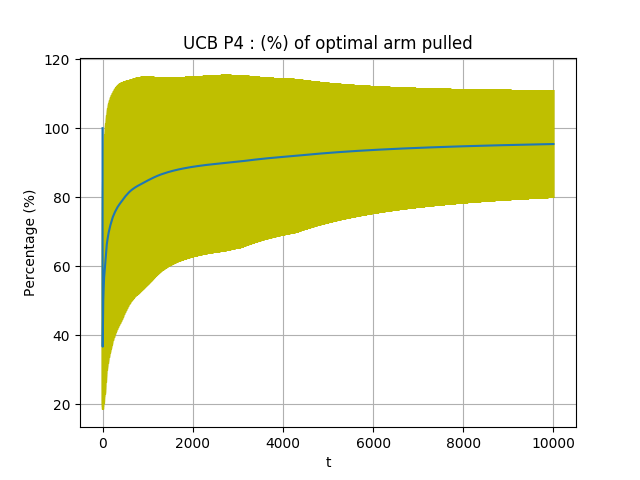
\includegraphics[scale=0.5]{Figures/UCB_P4_op.png} \par
					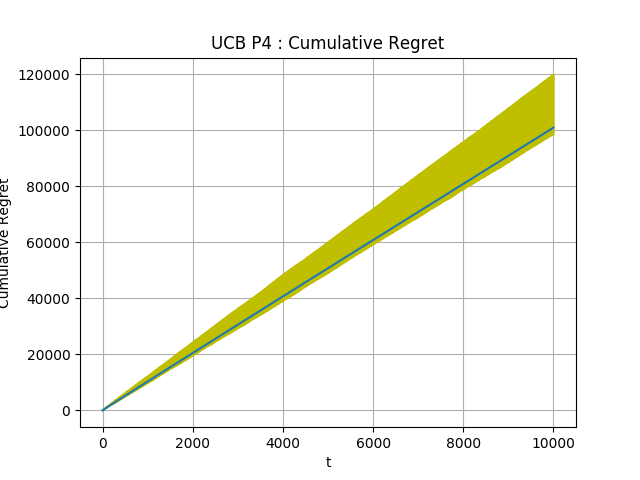
\includegraphics[scale=0.5]{Figures/UCB_P4_ret.png}
				\end{multicols}
				\caption{Evaluation plots for UCB for P4 set of arms}
				\label{Fig7}
			\end{figure}	
			
		\noindent On comparison, we see that at t=n, the percentage of optimal arms pulled by using ETC exceeds UCB by around $5\%$	but the final cumulative regret of ETC and UCB is almost same. So inorder to find which algorithm performs better in this case, let's analyse the figures showing percentage of optimal arm pulled. We seem that ETC identifies the optimal arm and almost completely exploits it. We see that the optimal m value is just 8 in this case. Hence exploitation happens in a very efficient manner and we get better rewards. And hence, in this case ETC outperforms UCB.
			

\section{Comparison of algorithms}
		\subsection{P1 set of Arms}
			\begin{figure}[H]
				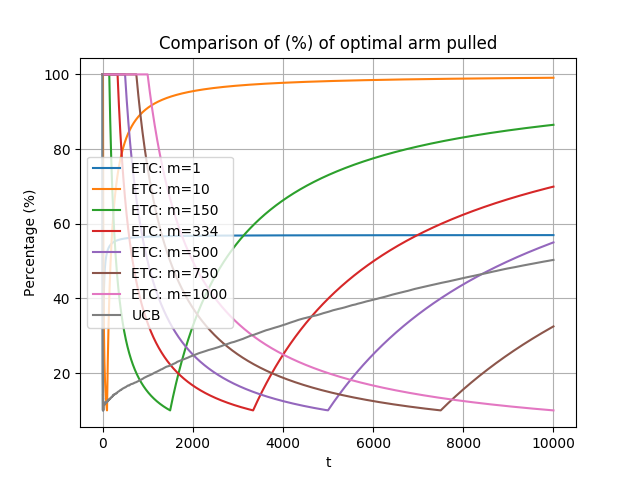
\includegraphics[scale=0.8]{Figures/Combined_op_P1.png}
				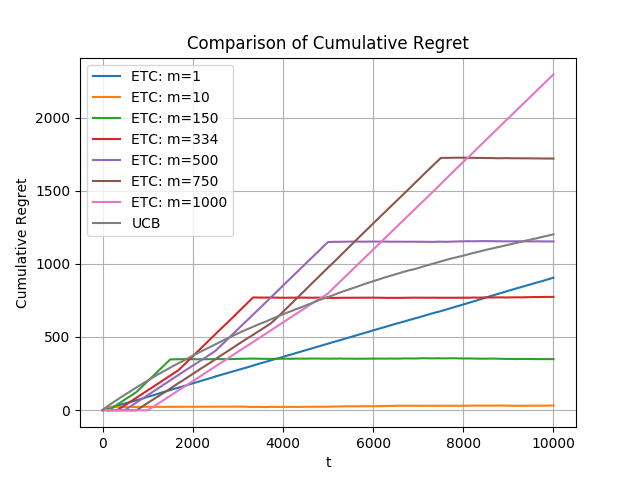
\includegraphics[scale=0.8]{Figures/Combined_regret_P1.png}
			\end{figure}
		
		\noindent Here, we see that ETC with $m = 10$ seems to be outperforming the others in the figure for percentage of optimal arm pulled. As m is increased (except for m=1), there is a general decrease in the performance of ETC algorithm in this figure. This is because we're exploring more and exploiting less. With smaller values of m from the optimal m, ETC performs better than UCB as can be seem from the first figure. But when it comes to final cumulative regret, the opposite is observed. ETC with larger values of m have better final regret values than UCB. But we also have to remember that there is randomness involved while sampling for the experiment.
		
		\subsection{P2 set of Arms}
			\begin{figure}[H]
				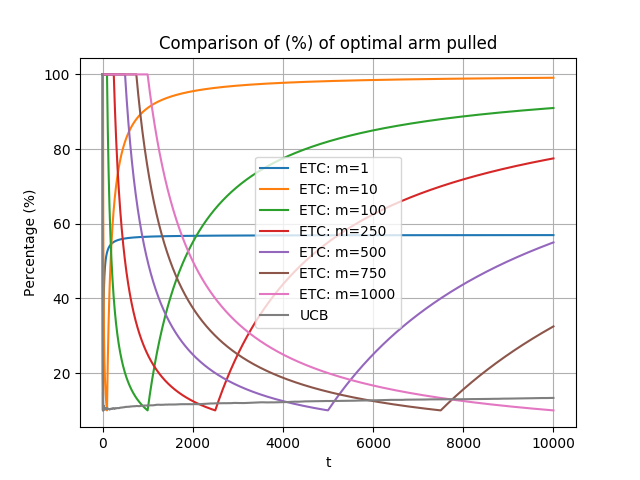
\includegraphics[scale=0.85]{Figures/Combined_op_P2.png}
				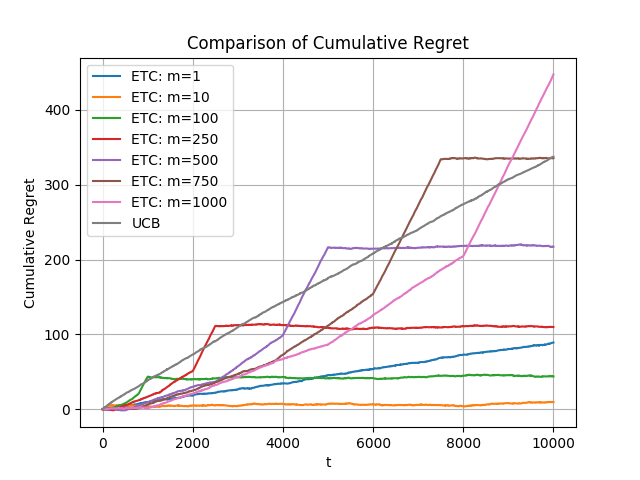
\includegraphics[scale=0.85]{Figures/Combined_regret_P2.png}
			\end{figure}
			
		\noindent Here, we see that ETC with $m = 10$ seems to be outperforming the others in the figure for percentage of optimal arm pulled. As m is increased (except for m=1), there is a general decrease in the performance of ETC algorithm in this figure. This is because we're exploring more and exploiting less. Here we see that, ETC outperforms UCB for all values of m (except m=1000) as can be seem from the first figure. But when it comes to final cumulative regret, ETC with larger values of m have better final regret values than UCB. But we also have to remember that there is randomness involved while sampling for the experiment.\\\\
		
		\noindent The reson for the ambiguity is same as that mentioned before in the case of P2. The mean values are extremely close and all the arms follow the same distribution (Bernoulli) and hence UCB performs very poorly in this case. On the other hand, even though the horizon is not sufficient to find an optimal m, ETC seems to perform fairly well. But then again in this case, because of close values of mean, the sub-optimal solutions found by UCB are not that bad.
		
		\subsection{P3 set of Arms}
			\begin{figure}[H]
				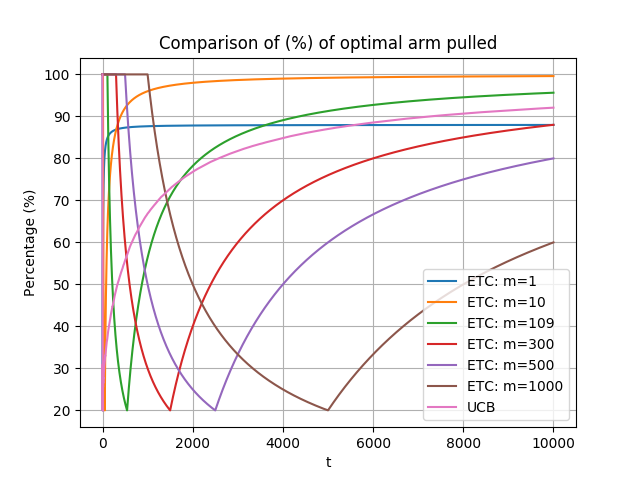
\includegraphics[scale=0.85]{Figures/Combined_op_P3.png}
				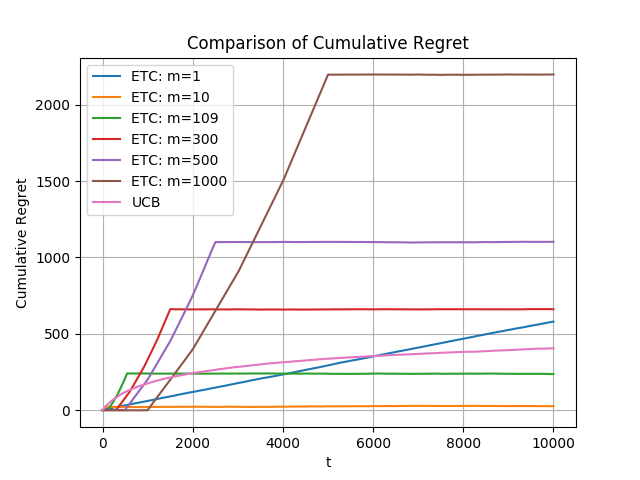
\includegraphics[scale=0.85]{Figures/Combined_regret_P3.png}
			\end{figure}
			
		\noindent Here, we see that ETC with $m = 10$ seems to be outperforming the others in the figure for percentage of optimal arm pulled. As m is increased (except for m=1), there is a general decrease in the performance of ETC algorithm in this figure. This is because we're exploring more and exploiting less. With smaller values of m from the optimal m, ETC performs better than UCB as can be seem from the first figure. But when it comes to final cumulative regret, the opposite is observed. ETC with larger values of m have better final cumulative regret values than UCB. So here we see a big trade-off between the percentage of optimal arms puutlled and the cumulative return at the end of the horizon while analysing the values of m. But in general in this case, ETC performs better than UCB.
		
		\subsection{P4 set of Arms}
			\begin{figure}[H]
				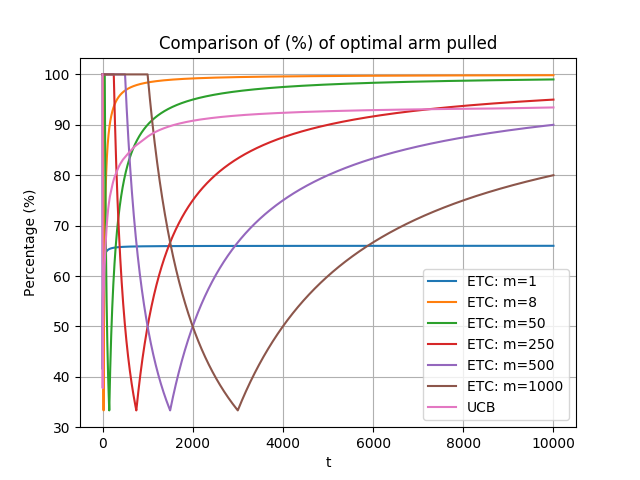
\includegraphics[scale=0.85]{Figures/Combined_op_P4.png}
				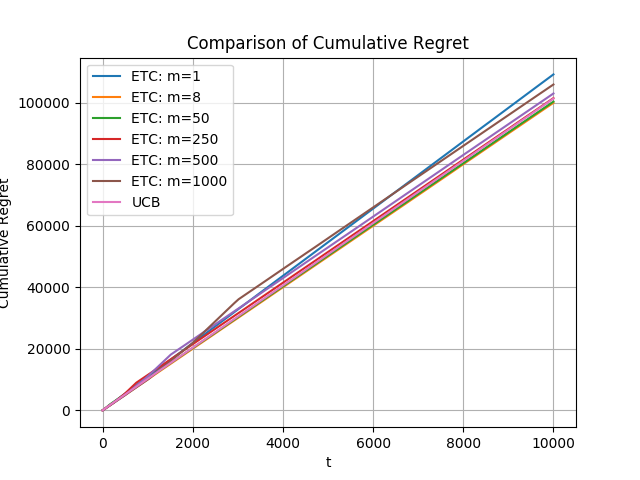
\includegraphics[scale=0.85]{Figures/Combined_regret_P4.png}
			\end{figure}
			g to be outperforming the others in the figure for percentage of optimal arm pulled. As m is increased (except for m=1), there is a general decrease in the performance of ETC algorithm in this figure. This is because we're exploring more and exploiting less. With small values of m, ETC performs better than UCB as can be seem from the first figure. But when it comes to final cumulative regret, ETC with larger values of m (except for m=1) have slightly better final cumulative regret values than UCB. But in general in this case, ETC performs better than UCB.
			
%-------------------------------------------------------------------------------
% REFERENCES
%------------------------------------------------------------------------ -------
\begin{thebibliography}{9}
\bibitem{1} 
Prof. Prashanth L. A. \textit{CS6046: Multi-armed bandits: Course notes}, 
Indian Institute of Technology Madras, March 19, 2018

\bibitem{2}
https://www.desmos.com/calculator
\end{thebibliography}


\end{document}

%-------------------------------------------------------------------------------
% SNIPPETS
%-------------------------------------------------------------------------------

%\begin{figure}[!ht]
%	\centering
%	\includegraphics[width=0.8\textwidth]{file_name}
%	\caption{}
%	\centering
%	\label{label:file_name}
%\end{figure}

%\begin{figure}[!ht]
%	\centering
%	\includegraphics[width=0.8\textwidth]{graph}
%	\caption{Blood pressure ranges and associated level of hypertension (American Heart Association, 2013).}
%	\centering
%	\label{label:graph}
%\end{figure}

%\begin{wrapfigure}{r}{0.30\textwidth}
%	\vspace{-40pt}
%	\begin{center}
%		\includegraphics[width=0.29\textwidth]{file_name}
%	\end{center}
%	\vspace{-20pt}
%	\caption{}
%	\label{label:file_name}
%\end{wrapfigure}

%\begin{wrapfigure}{r}{0.45\textwidth}
%	\begin{center}
%		\includegraphics[width=0.29\textwidth]{manometer}
%	\end{center}
%	\caption{Aneroid sphygmomanometer with stethoscope (Medicalexpo, 2012).}
%	\label{label:manometer}
%\end{wrapfigure}

%\begin{table}[!ht]\footnotesize
%	\centering
%	\begin{tabular}{cccccc}
%	\toprule
%	\multicolumn{2}{c} {Pearson's correlation test} & \multicolumn{4}{c} {Independent t-test} \\
%	\midrule	
%	\multicolumn{2}{c} {Gender} & \multicolumn{2}{c} {Activity level} & \multicolumn{2}{c} {Gender} \\
%	\midrule
%	Males & Females & 1st level & 6th level & Males & Females \\
%	\midrule
%	\multicolumn{2}{c} {BMI vs. SP} & \multicolumn{2}{c} {Systolic pressure} & \multicolumn{2}{c} {Systolic Pressure} \\
%	\multicolumn{2}{c} {BMI vs. DP} & \multicolumn{2}{c} {Diastolic pressure} & \multicolumn{2}{c} {Diastolic pressure} \\
%	\multicolumn{2}{c} {BMI vs. MAP} & \multicolumn{2}{c} {MAP} & \multicolumn{2}{c} {MAP} \\
%	\multicolumn{2}{c} {W:H ratio vs. SP} & \multicolumn{2}{c} {BMI} & \multicolumn{2}{c} {BMI} \\
%	\multicolumn{2}{c} {W:H ratio vs. DP} & \multicolumn{2}{c} {W:H ratio} & \multicolumn{2}{c} {W:H ratio} \\
%	\multicolumn{2}{c} {W:H ratio vs. MAP} & \multicolumn{2}{c} {\% Body fat} & \multicolumn{2}{c} {\% Body fat} \\
%	\multicolumn{2}{c} {} & \multicolumn{2}{c} {Height} & \multicolumn{2}{c} {Height} \\
%	\multicolumn{2}{c} {} & \multicolumn{2}{c} {Weight} & \multicolumn{2}{c} {Weight} \\
%	\multicolumn{2}{c} {} & \multicolumn{2}{c} {Heart rate} & \multicolumn{2}{c} {Heart rate} \\
%	\bottomrule
%	\end{tabular}
%	\caption{Parameters that were analysed and related statistical test performed for current study. BMI - body mass index; SP - systolic pressure; DP - diastolic pressure; MAP - mean arterial pressure; W:H ratio - waist to hip ratio.}
%	\label{label:tests}
%\end{table}